\chapter{Retrospect}
In this chapter, the objective is to evaluate all of the choices the team has made during the project. This includes the time spent, the entire development process - from choosing IDEs to testing the system and the project management. 


\input ch/retrospect/sec/timespent.tex
\input ch/retrospect/sec/inflRisks.tex
\input ch/retrospect/sec/workStructure.tex

\subsection{Improper use of Yodiz}
\label{sec:improperScrum}
As mentioned in section~\ref{sec:scrumtool}, the team used a lot of time on
deciding on which Scrum tool to use for the project management. Although our
choice fell on Yodiz, the team was in lack of any previous experience with the
tool, and despite the team's efforts to get acquainted with the tool, a
misunderstanding arose and was not discovered until the end of the second
sprint.

The misunderstanding, displayed in figure~\ref{fig:wrongUse}, was that the team
assumed one could add multiple individuals as responsible on a particular task,
while Yodiz' functionality only assigned the time spent to the individual that
either created the task or was assigned as owner of the task.

As a result, it appeared as if only singular individuals performed the tasks,
even though the entire team in reality was participating, which was also
reflected in the burn down charts and the generated Gantt diagram. 

To sort out this issue, the team went through old meeting reports and time sheets
to figure out which members of the team that had actually participated on the
particular task, and added new tasks and the time spent to the members that at
the time had not recorded this information.%, as shown in figure~\ref{fig:addsTasks}.

This issue was unfortunate, but not insurmountable, and also not a critical
issue for the overall progress of the project.

\begin{figure}[H]
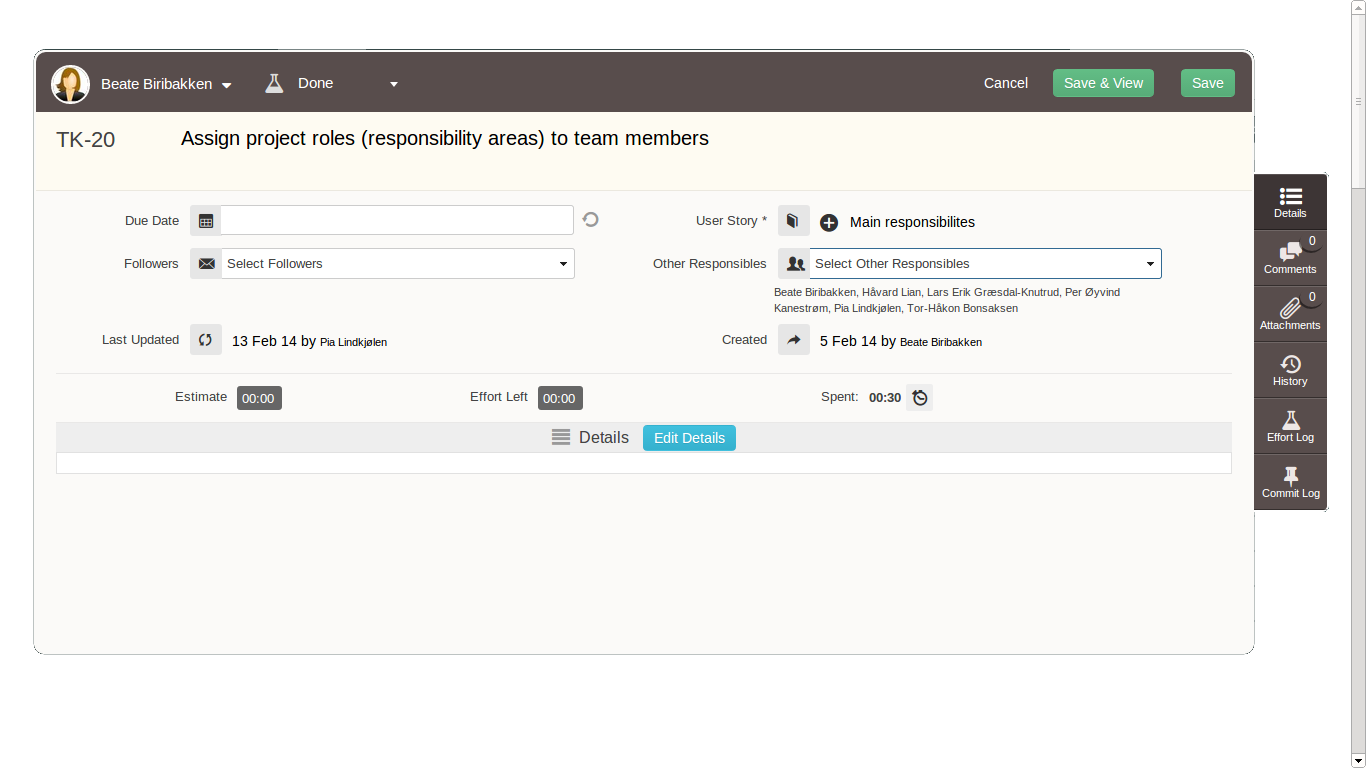
\includegraphics[width=\textwidth, clip, trim=1cm 2cm 4cm 1cm]{ch/retrospect/fig/wrongUse.png}
\caption{Example screenshot to illustrate improper use of Yodiz}
\label{fig:wrongUse}
\end{figure}

\begin{comment}
not sure if this is necessary
\begin{figure}[H]
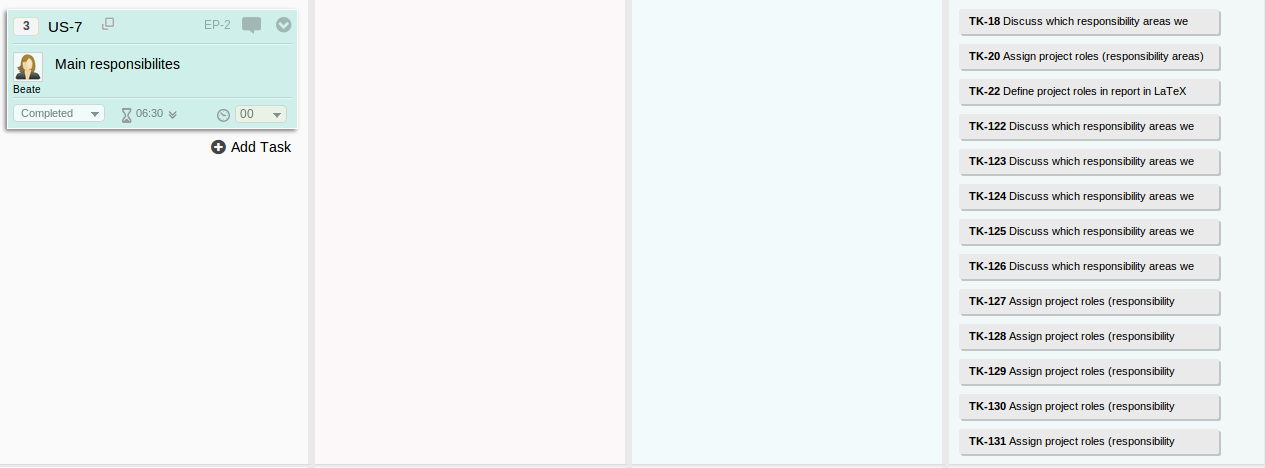
\includegraphics[width=\textwidth]{ch/retrospect/fig/addsTasks.png}
\caption{Example screenshot to illustrate how the team resolved the issue.}
\label{fig:addsTasks}
\end{figure}
\end{comment}


\section{Development process}
In this section all of the problems and solutions related to the development process will be discussed and evaluated. This involves problems related to scrum, to the team organization and the technical choices the team has made during the project. 

\subsection{Scrum and extreme programming}

The team chose to use scrum together with extreme programming. This process and why these were chosen is described in section ~\ref{sec:scrumDevProcess}. Even though Scrum is well known, many team members had different expectations to how the framework would be implemented in the project.


OMFORMULERES: Each team member spent a significant amount of time getting up to date with the Android platform and the front-end architecture of Android apps. In retrospect, more time should have been spent getting all group members up to date and practicing Android programming together in the beginning of the project. One of the team members had some experience with Android before and ended up spending a lot of time teaching and explaining to all of the other team members. If this had been organized in a way, for instance by holding a course in the beginning, some of the time spent on this could have been saved. 

\subsection{Technical choices}
The team agreed on using Android studio from the beginning, after discussing whether to use Android studio or eclipse with an Android plugin. In the beginning there were some problems with Android Studio. Some team members had trouble actually running the app. There was a problem with Android Studio not finding the correct SDK. (<-IS THIS CORRECT?) This took some time to solve, but after it was solved the team had no more trouble with is. However, since Android Studio is a relatively new IDE, is still has some start trouble and updates comes out regularly. This meant that all of the group members had to use at least two or three minutes every time a new update came out. 

We changed the architecture during the process, we should write about that and why here, do we think we chose the best one? We chose to create a provider, do we feel it was worth all the extra time it took? 

\subsubsection{Choice of Android IDE}
Despite the fact that some the team members already had experience with Android Studio's counterpart Eclipse ADT, and few of us had any experience with Android Studio, the team wanted to give it a try, as it appeared to have more features, such as a faster compiler, better search function and auto completion of code, than Eclipse ADT. 

As the project has progressed, it has become clear that the learning curve has not been as steep as expected. Neither have we encountered any problems that we did not think also would have been present if we had chosen to use Eclipse ADT.

\subsubsection{Choice of GitHub for code management}
By taking the customer's opinion in this matter into consideration, we were be more able to give the customer a better overview of the project and also to easily integrate our app into the customer's existing project. As a result, both the team and the customer were updated on the last version of the project and the team was more likely to receive relevant feedback. 

\section{Project management}
SECTION NOT FINISHED. As mentioned earlier, the team chose scrum. Yodiz, we now wish we had chose another scrum tool. After a while we added a person responsible for some serving on our work days. Also responsible for making sure we took brakes. 
The team introduced punishments for being to late for meetings and not doing all of your assignments. This was used on a team building with some food. Did this work optimally?
\subsection{Working with the customer}
SECTION NOT FINISHED. The team tried to have meetings with the customer once a week. This worked well and the team felt that it was a good thing that the customer participated to such an extent. Write something about the problems with the customer saying he is going to do something but did not and how we solved the problems around this?

\subsection{Team organization}
SECTION NOT FINISHED.
In the beginning of the project, the team distributed roles with different responsibilities. A project leader, a deputy project leader, a scrum master, a development responsible, a test responsible and a report responsible. Almost halfway through the project it became clear that the scrum master was also the one with the most Android experience. This resulted in a lot of extra work on the scrum master, while the deputy project leader had almost no work at all. Therefore, the team reflected over the project roles and the distribution and this resulted in a change of roles. The deputy project leader became the scrum master to distribute the resources in the best possible way. After this change the teams best Android resource could focus entirely on developing and helping others. The team was very satisfied with this decision and the resource distribution worked great after the change in roles. 

Was the responsibilities of the roles good?
